\documentclass[10pt,leqno]{article}
\usepackage{comment}
%auto-ignore
%!TEX root = webs.tex
%this ensures the arxiv doesn't try to start TeXing here.

\usepackage{amsmath,amssymb,amsfonts,amsthm}
\usepackage{ifpdf}

\usepackage{comment}

\usepackage[all]{xy}
\SelectTips{cm}{}
% This may speed up compilation of complex documents with many xymatrices.
%\CompileMatrices

\usepackage[section]{placeins}
\usepackage{leftidx}
\usepackage{stmaryrd} % additional math symbols, e.g. \mapsfrom
%\usepackage{libertine}
%\usepackage[T1]{fontenc}
\usepackage{microtype}

% ----------------------------------------------------------------
\vfuzz5pt % Don't report over-full v-boxes if over-edge is small
\hfuzz5pt % Don't report over-full h-boxes if over-edge is small
% ----------------------------------------------------------------

% don't warn about PDF 1.5 (default was 1.4); dangerous?
\pdfminorversion=5

% diagrams -------------------------------------------------------
% figures ---------------------------------------------------------
\newcommand{\pathtotrunk}{./}
\newcommand{\pathtodiagrams}{\pathtotrunk}

\newcommand{\mathfig}[2]{\ensuremath{\hspace{-3pt}\begin{array}{c}%
  \raisebox{-2.5pt}{\includegraphics[width=#1\textwidth]{\pathtodiagrams #2}}%
\end{array}\hspace{-3pt}}}
\newcommand{\reflectmathfig}[2]{{\hspace{-3pt}\begin{array}{c}%
  \raisebox{-2.5pt}{\reflectbox{\includegraphics[width=#1\textwidth]{\pathtodiagrams #2}}}%
\end{array}\hspace{-3pt}}}
\newcommand{\rotatemathfig}[3]{{\hspace{-3pt}\begin{array}{c}%
  \raisebox{-2.5pt}{\rotatebox{#2}{\includegraphics[height=#1\textwidth]{\pathtodiagrams #3}}}%
\end{array}\hspace{-3pt}}}
\newcommand{\placefig}[2]{\includegraphics[width=#1\linewidth]{\pathtodiagrams #2}}

\newcommand{\arxiv}[1]{\href{http://arxiv.org/abs/#1}{\tt arXiv:\nolinkurl{#1}}}
\newcommand{\doi}[1]{\href{http://dx.doi.org/#1}{{\tt DOI:#1}}}
\newcommand{\euclid}[1]{\href{http://projecteuclid.org/euclid.cmp/#1}{{\tt #1}}}
\newcommand{\mathscinet}[1]{\href{http://www.ams.org/mathscinet-getitem?mr=#1}{\tt #1}}
\newcommand{\googlebooks}[1]{(preview at \href{http://books.google.com/books?id=#1}{google books})}


% THEOREMS -------------------------------------------------------
\theoremstyle{plain}
%\newtheorem*{fact}{Fact}
\newtheorem{prop}{Proposition}[subsection]
\makeatletter
\@addtoreset{prop}{section}
\makeatother
\newtheorem{conj}[prop]{Conjecture}
\newtheorem{thm}[prop]{Theorem}
\newtheorem{lem}[prop]{Lemma}
\newtheorem*{lem*}{Lemma}
\newtheorem{cor}[prop]{Corollary}
\newtheorem*{cor*}{Corollary}
\newtheorem*{exc}{Exercise}
\newtheorem{defn}[prop]{Definition}         % numbered definition
\newtheorem*{defn*}{Definition}             % unnumbered definition
\newtheorem{question}{Question}
\newtheorem{property}[prop]{Property}
\newenvironment{rem}{\vspace{0.3cm}\noindent\textsl{Remark.}}{}  % perhaps looks better than rem above?
\newenvironment{example}{\vspace{0.3cm}\noindent\textbf{Example.}}{}  % perhaps looks better than rem above?
\newtheorem{rem*}[prop]{Remark}
\numberwithin{equation}{section}
%% example, claim and remark are defined in article_preamble.tex, for compatibility with beamer and PNAS


% Marginal notes in draft mode -----------------------------------
\newcounter{comment}
\newcommand{\noop}[1]{}
\newcommand{\todo}[1]{\textbf{\color[rgb]{.8,.2,.5}\small TODO: #1}}

% \mathrlap -- a horizontal \smash--------------------------------
% For comparison, the existing overlap macros:
% \def\llap#1{\hbox to 0pt{\hss#1}}
% \def\rlap#1{\hbox to 0pt{#1\hss}}
\def\clap#1{\hbox to 0pt{\hss#1\hss}}
\def\mathllap{\mathpalette\mathllapinternal}
\def\mathrlap{\mathpalette\mathrlapinternal}
\def\mathclap{\mathpalette\mathclapinternal}
\def\mathllapinternal#1#2{%
\llap{$\mathsurround=0pt#1{#2}$}}
\def\mathrlapinternal#1#2{%
\rlap{$\mathsurround=0pt#1{#2}$}}
\def\mathclapinternal#1#2{%
\clap{$\mathsurround=0pt#1{#2}$}}

% MATH -----------------------------------------------------------
\newcommand{\id}{\boldsymbol{1}}
\renewcommand{\imath}{\mathfrak{i}}
\renewcommand{\jmath}{\mathfrak{j}}

\newcommand{\ssum}[1]{\Sigma#1}
\newcommand{\sumhat}{\overline{\sum}}
\newcommand{\sumtah}{\underline{\sum}}

\newcommand{\lmod}[1]{\leftidx{_{#1}}{\operatorname{mod}}{}}

\newcommand{\into}{\hookrightarrow}
\newcommand{\onto}{\twoheadrightarrow}
\newcommand{\iso}{\cong}
\newcommand{\quism}{\underset{\text{q.i.}}{\simeq}}
\newcommand{\htpy}{\simeq}
\newcommand{\actsOn}{\circlearrowright}
\newcommand{\xto}[1]{\xrightarrow{#1}}
\newcommand{\isoto}{\xto{\iso}}
\newcommand{\quismto}{\xrightarrow[\text{q.i.}]{\iso}}
\newcommand{\diffeoto}{\xrightarrow[\text{diffeo}]{\iso}}
\newcommand{\htpyto}{\xrightarrow[\text{htpy}]{\htpy}}

\newcommand{\restrict}[2]{#1{}_{\mid #2}{}}
\newcommand{\set}[1]{\left\{#1\right\}}
\newcommand{\setc}[2]{\setcl{#1}{#2}}
\newcommand{\setcl}[2]{\left\{ \left. #1 \;\right| \; #2 \right\}}
\newcommand{\setcr}[2]{\left\{ #1 \;\left| \; #2 \right\}\right.}

\newcommand{\floor}[1]{\left\lfloor#1\right\rfloor}
\newcommand{\norm}[1]{\left|\left|#1\right|\right|}
\newcommand{\abs}[1]{\left|#1\right|}

\newcommand{\qi}[2][q]{\left[#2\right]_{#1}}
\newcommand{\qBinomial}[3][q]{\genfrac{[}{]}{0pt}{}{#2}{#3}_{#1}}
\newcommand{\qPoch}[3]{\left(#1;#2\right)_{#3}}

\newcommand{\card}[1]{\sharp{#1}}

\newcommand{\bdy}{\partial}
\newcommand{\compose}{\circ}
\newcommand{\eset}{\emptyset}

\newcommand{\directSum}{\oplus}
\newcommand{\DirectSum}{\bigoplus}
\newcommand{\tensor}{\otimes}
\newcommand{\Tensor}{\bigotimes}

\newcommand{\Homa}[3]{\Hom_{#1}\left(#2,#3\right)}
\newcommand{\Hom}{\operatorname{Hom}}
\newcommand{\End}[1]{\operatorname{End}\left(#1\right)}

% ----------------------------------------------------------------

\ifpdf
	\usepackage[pdftex,plainpages=false,hypertexnames=false,pdfpagelabels]{hyperref}
	\usepackage[pdftex]{graphicx}
\else
	\usepackage[plainpages=false,hypertexnames=false,pdfpagelabels]{hyperref}
	\usepackage{graphicx}
\fi

%must load tikz after graphicx
\usepackage{tikz}
\usetikzlibrary{shapes}
\usetikzlibrary{backgrounds}
\usetikzlibrary{decorations,decorations.pathreplacing,decorations.markings}
\usetikzlibrary{fit,calc,through}
\usetikzlibrary{external}

\tikzstyle{mid>}=[decoration={markings, mark=at position 0.5 with {\arrow{>}}}, postaction={decorate}]
\tikzstyle{mid<}=[decoration={markings, mark=at position 0.5 with {\arrow{<}}}, postaction={decorate}]
\tikzstyle{upper>}=[decoration={markings, mark=at position 0.8 with {\arrow{>}}}, postaction={decorate}]
\tikzstyle{upper<}=[decoration={markings, mark=at position 0.8 with {\arrow{<}}}, postaction={decorate}]
\tikzstyle{lower>}=[decoration={markings, mark=at position 0.2 with {\arrow{>}}}, postaction={decorate}]
\tikzstyle{lower<}=[decoration={markings, mark=at position 0.2 with {\arrow{<}}}, postaction={decorate}]

\def\Foam{{\mathcal{F}{\rm oam}}}
\newcommand{\alt}{\wedge}
\newcommand{\Alt}[2]{{\textstyle\bigwedge^{#1}_{#2}}}
\newcommand{\Usl}[1]{U\sl_{#1}}
\newcommand{\one}{1}
\def\sA{\mathcal{A}}
\def\l{\lambda}
\def\bZ{{\mathbb{Z}}}
\def\sl{{\mathfrak{sl}}}
\def\Sp{{\mathcal{S}p}}
\def\FSp{{\mathcal{FS}p}}
\def\bC{{\mathbb{C}}}
\def\g{{\mathfrak{g}}}
\def\SL{{\rm{SL}}}
\def\GL{{\rm{GL}}}
\def\gl{{\mathfrak{gl}}}
\def\dU{\dot{{\mathcal{U}}}_q}
\def\Uq{\mathcal{U}_q}
\def\Rep{\mathcal{R}ep}
\def\la{\langle}
\def\ra{\rangle}
\def\dalg{\dot{{U}}_q}

\newcommand{\ul}[1]{{\underline{#1}}}

%\newcommand{\RepSL}[1]{\mathcal{R}ep(SL_{#1})}
\newcommand{\Lad}{\mathcal{L}ad}

\usepackage{environ}
\usepackage{xargs}

\newcommandx{\NewEnvironx}[5][2,3]{%
  \expandafter\newcommandx\csname start#1\endcsname[#2][#3]{#4}%
  \NewEnviron{#1}{\csname start#1\expandafter\endcsname\BODY #5}}

\newcommand{\ladderX}{1.5}
\newcommand{\ladderY}{1.5}
\newcommand{\ladderR}{0.6}
\newcommand{\laddercoordinates}[2]{
\foreach \x in {0,...,#1} {
	\foreach \y in {0,...,#2} {
		\coordinate (l\x\y) at (\x * \ladderX, \y * \ladderY);
		\coordinate (u\x\y) at ($(l\x\y)+\ladderR*(0,\ladderY)$);
		\coordinate (d\x\y) at ($(l\x\y)+(0,\ladderY)-\ladderR*(0,\ladderY)$);
	}
}
}
\newcommand{\ladderEn}[5]{
\draw[mid>] (l#1#2) -- (d#1#2);
\draw[mid>] (d#1#2) -- ($(l#1#2)+(0,\ladderY)$) node[left] {#3};
\draw[mid>] ($(l#1#2)+(\ladderX,0)$) -- ($(u#1#2)+(\ladderX,0)$);
\draw[mid>] ($(u#1#2)+(\ladderX,0)$) -- ($(l#1#2)+(\ladderX,\ladderY)$) node[right] {#4};
\draw[mid>] (d#1#2) --node[above]{#5} ($(u#1#2)+(\ladderX,0)$);
}
\newcommand{\ladderE}[4]{\ladderEn{#1}{#2}{#3}{#4}{}}
\newcommand{\ladderFn}[5]{
\draw[mid>] (l#1#2) -- (u#1#2);
\draw[mid>] (u#1#2) -- ($(l#1#2)+(0,\ladderY)$) node[left] {#3};
\draw[mid>] ($(l#1#2)+(\ladderX,0)$) -- ($(d#1#2)+(\ladderX,0)$);
\draw[mid>] ($(d#1#2)+(\ladderX,0)$) -- ($(l#1#2)+(\ladderX,\ladderY)$) node[right] {#4};
\draw[mid>] ($(d#1#2)+(\ladderX,0)$) --node[above]{#5} (u#1#2);
}
\newcommand{\ladderF}[4]{\ladderFn{#1}{#2}{#3}{#4}{}}
\newcommand{\ladderIn}[3]{\draw[mid>] (l#1#2) -- +($#3*(0,\ladderY)$);}
\newcommand{\ladderI}[2]{\ladderIn{#1}{#2}{1}}

\NewEnvironx{ladder}[2]{%
  \begin{tikzpicture}[baseline=13*\ladderY*#2]\laddercoordinates{#1}{#2}}
{\end{tikzpicture}}

\newcommand{\fuse}[3]{\tikz[baseline=0.5cm]{
\coordinate (z1) at (0,0);
\coordinate (z2) at (1,0);
\coordinate (c) at (0.5,0.5);
\coordinate (e) at (0.5,1);
\draw[mid>] (z1) node[below] {$#1$} -- (c);
\draw[mid>] (z2) node[below] {$#2$} -- (c);
\draw[mid>] (c) -- (e) node[above] {$#3$};
}}
\newcommand{\fork}[3]{\tikz[baseline=0.5cm]{
\coordinate (z1) at (0,1);
\coordinate (z2) at (1,1);
\coordinate (c) at (0.5,0.5);
\coordinate (e) at (0.5,0);
\draw[mid<] (z1) node[above] {$#1$} -- (c);
\draw[mid<] (z2) node[above] {$#2$} -- (c);
\draw[mid<] (c) -- (e) node[below] {$#3$};
}}


% example for creating tikz environments compatible with externalize
% thanks Andrew Stacey: http://tex.stackexchange.com/a/15614/77
%\NewEnvironx{mytikz}[1][1=]{%
%  \begin{figure}[htp]
%  \centering
%  \begin{tikzpicture}[#1]}
%{\end{tikzpicture}
%  \end{figure}}

% tricky way to iterate macros over a list
\def\semicolon{;}
\def\applytolist#1{
    \expandafter\def\csname multi#1\endcsname##1{
        \def\multiack{##1}\ifx\multiack\semicolon
            \def\next{\relax}
        \else
            \csname #1\endcsname{##1}
            \def\next{\csname multi#1\endcsname}
        \fi
        \next}
    \csname multi#1\endcsname}

% \def\cA{{\cal A}} for A..Z
\def\calc#1{\expandafter\def\csname c#1\endcsname{{\mathcal #1}}}
\applytolist{calc}QWERTYUIOPLKJHGFDSAZXCVBNM;

\usepackage{color}

% idea from tex-overflow
\usepackage{xcolor}
\definecolor{dark-red}{rgb}{0.7,0.25,0.25}
\definecolor{dark-blue}{rgb}{0.15,0.15,0.55}
\definecolor{medium-blue}{rgb}{0,0,0.65}
\hypersetup{
    colorlinks, linkcolor={dark-red},
    citecolor={dark-blue}, urlcolor={medium-blue}
}


% margin stuff
\setlength{\textwidth}{6.5in}
\setlength{\oddsidemargin}{0in}
\setlength{\evensidemargin}{0in}
\setlength{\textheight}{8.5in}
\setlength{\topmargin}{-.25in}



%\tikzexternalize[prefix=diagrams/externalized/]


\title{something about webs and skew Howe duality}
\author{Sabin~Cautis, Joel~Kamnitzer and Scott~Morrison}

\begin{document}

\makeatletter
\@addtoreset{equation}{section}
\gdef\theequation{\thesection.\arabic{equation}}
\makeatother

\maketitle

\begin{abstract}
\end{abstract}

\hypersetup{
    colorlinks, linkcolor={black},
    citecolor={dark-blue}, urlcolor={medium-blue}
}

\tableofcontents

\hypersetup{
    colorlinks, linkcolor={dark-red},
    citecolor={dark-blue}, urlcolor={medium-blue}
}

\newcommand{\alt}{\wedge}

\newcommand{\Alt}{\bigwedge}

\newcommand{\Usl}[1]{U\sl_{#1}}

\newcommand{\one}{1}

\def\sl{{\mathfrak{sl}}}
\def\Sp{{\mathcal{S}p}}
\def\FSp{{\mathcal{FS}p}}
\def\bC{{\mathbb{C}}}
\def\g{{\mathfrak{g}}}
\def\SL{{\rm{SL}}}
\def\GL{{\rm{GL}}}
\def\gl{{\mathfrak{gl}}}
\def\dU{\dot{{\mathcal{U}}}}
\def\Rep{\mathcal{R}ep}
\def\la{\langle}
\def\ra{\rangle}
% \newcommand{\gl}[1]{\mathfrak{gl}_{#1}}
%\newcommand{\Ugl}[1]{U\gl{#1}}

\newcommand{\ul}[1]{{\underline{#1}}}

%\newcommand{\RepSL}[1]{\mathcal{R}ep(SL_{#1})}
\newcommand{\Lad}{\mathcal{L}ad}

\section{Introduction}
The representation theory of $\sl_n$ is a pivotal tensor category, and it is natural to ask for a presentation by generators and relations, as a pivotal tensor category.

There are two main choices one needs to make before looking for such a presentation. First, it would be reasonable to pass to any full subcategory, whose idempotent completion recovers the entire representation theory. In particular, in this paper we look at the full subcategory (denoted $\Rep(\SL_n)$) whose objects are isomorphic to tensor products of the fundamental representations $\Alt^k \mathbb C^n$ of $\sl_n$. (It might alternatively be interesting to descend all the way to the full subcategory whose objects are tensor powers of the standard representation.) Second, we need to decide which generators to use. We take the maps $\Alt^a \mathbb{C}^n \tensor \Alt^b \mathbb{C}^n \tensor \Alt^c \mathbb{C}^n \to \mathbb{C}$. (The space of such maps is one-dimensional if $a+b+c$ is a multiple of $n$, or zero-dimensional otherwise.) It is relatively easy to show that these are indeed generators, i.e. that every $\sl_n$-linear map between tensor products of fundamental representations can be written as tensor products and compositions of these maps, along with the duality pairing and copairing maps \cite[Proposition 3.5.8]{0704.1503}. The question then, is to identify the relations holding between such planar compositions.

Said another way, we have a pivotal category of trivalent webs, with oriented edges labelled by $\{1, \ldots, n-1\}$, and at each vertex the labels summing to a multiple of $n$, and a full and dominant functor to the representation theory category. The question is to identify the pivotal ideal which is the kernel of this functor.

This problem has been studied previously. For $n=2$, there are no trivalent vertices, and the category of webs is essentially just the category of embedded 1-manifolds up to isotopy. The kernel of the functor to representation theory is the ideal generated by the difference $\tikz[baseline=-2pt]{\node[draw,circle] {};} - 2$. \todo{Explain that this is Temperley-Lieb.}

For $n=3$ .... \todo{talk about Kuperberg's relations for $\sl_3$ \cite{MR1403861}.}

For $n \geq 4$, generators for the kernel have been proposed, by \cite{math.QA/0310143} (for $n=4$) and by \cite{0704.1503} (generally), but without proving that their lists of relations were complete.

This paper answers the question, in particular showing that the relations of \cite{0704.1503} are complete. In fact, those relations are over complete; just the $I=H$ and `square-switch' relations suffice (and in fact only one of the square-switch relations implies the others), and generate the others. The relevant relations are reproduced in \S\ref{sec:diagrams}.
The main theorem, stating the isomorphism between a combinatorially defined web category and the representation theory of $\Usl{n}$, appears in \S \ref{sec:theorem}.

The core idea of our proof is to use skew Howe duality. In fact we give a very succinct recipe for the relations, as certain truncations of relations holding in $\Usl{m}$. We now give a quick overview of the argument.

We denote the quotient of the category of trivalent webs by the $I=H$ and square switch relations as $\Sp(SL_n)$. We have a surjective functor to the the representation theory, which we would like to show is an isomorphism. All that remains is to check that it is injective on morphisms.

Skew Howe duality states that the commuting actions of $\Usl{n}$ and $\Usl{m}$ on $\Alt^\bullet(\mathbb{C}^n \tensor \mathbb{C}^m)$ are in fact each the commutant of the other. That is, if  $f: \Alt^\bullet(\mathbb{C}^n \tensor \mathbb{C}^m) \to \Alt^\bullet(\mathbb{C}^n \tensor \mathbb{C}^m)$ is $\sl_n$-linear, then there is some element $X_f \in \Usl{m}$ whose action on  $\Alt^\bullet(\mathbb{C}^n \tensor \mathbb{C}^m)$ is exactly $f$.

Suppose we have some element $A \in \Homa{\Sp(SL_n)}{\underline{k}}{\underline{k'}}$ which maps to zero in the representation theory. Here $\underline{k}$ and $\underline{k}$ denote two sequences of integers with signs from the set $\{1^\pm,\ldots,n-1^\pm\}$, i.e. two objects in $\Sp(SL_n)$. (The sign indicates whether the strand and that boundary point is oriented up or down.) First, we realize that by conjugating $A$ by the isomorphisms between $k^-$ and $(n-k)^+$ in $\Sp(SL_n)$, which are sent to isomorphisms in the representation theory, we may assume that all the signs are positive.

 We would like to show that $A$ is itself zero. 
 We then choose sequences $\ul{l}$ and $\ul{l'}$ obtained from $\underline{k}$ by interposing some number of $0$s and $n$s, so $\ul{l}$ and $\ul{l'}$ have the same length $m$ and the same sum $L$ (previously, the sums of $\underline{k}$ and $\underline{k'}$ might be differed by a multiple of $n$).
 The element $A$ is then equivalent, via the specified relations in $\Sp(SL_n)$ to a `ladder diagram' with $m$ rails and boundary given by the sequences $\ul{l}$ and $\ul{l'}$. (See Figure \ref{fig:ladder-example} for an example.)
 \todo{an example ladder diagram}
A complete description of ladder diagrams and this equivalence to a ladder diagram is in \S \ref{sec:ladders}.

Now, rewriting $\Alt^L(\mathbb C^n \tensor \mathbb C^m)$ as
\begin{align*}
\alt^L(\mathbb C^n \tensor \mathbb C^m) & = \alt^L(\mathbb C^n \directSum \cdots \directSum \mathbb C^n) \\
        & = \DirectSum_{\underline{l}: \sum \underline{l} = L} \alt^{l_1} \mathbb C^n \tensor \cdots \tensor \alt^{l_m} \mathbb C^n
\end{align*}
we see the objects $\underline{l}$ and $\underline{l}'$ as summands, and hence $A$ as an endomorphism of $\Alt^L(\mathbb C^n \tensor \mathbb C^m)$. Thus there is some element $X_{A} \in \dU(\gl_m)$, which acts by zero on $\Alt^L(\mathbb C^n \tensor \mathbb C^m)$. In fact, since we had shown $A$ was equivalent to a ladder diagram, we can write down an explicit element $X_A$, by interpreting each rung of the ladder as some $E^{(a)}_j$ or $F^{(a)}_j$ in $\dU(\gl_m)$. 

Next, we find that we can explicitly describe the kernel of $\dU(\gl_m)$ acting on $\Alt^\bullet(\mathbb C^n \tensor \mathbb C^m)$. The kernel is precisely the ideal generated by those weight space idempotents falling outside the weight support of $\Alt^\bullet(\mathbb C^n \tensor \mathbb C^m)$. \todo{Saying this requires having previously mentioned the idempotented form.} This result is proved in \S \ref{sec:kernel}.


\section{The categories $\Rep(\SL_n)$ and $\Sp(\SL_n)$}\label{sec:diagrams}

We denote by $[n]_q$ the quantum integer $q^{n-1} + q^{n-3} + \dots + q^{-n+3} + q^{-n+1}$. More generally, 
$$\qBinomial{n}{k} := \frac{[n]_q\dots[1]_q}{([n-k]_q \dots [1]_q)([k]_q \dots [1]_q)}.$$
We will denote by $U_q(\sl_n)$ the quantum group associated to $\sl_n$. 

\subsection{Definition of the representation category $\Rep(\SL_n)$}

The objects in $\Rep(\SL_n)$ are tensor products of the fundamental representations $\alt^k \bC^n$ of $U_q(\sl_n)$. These are clearly in bijection with tuples $\ul{k} = (k_1, \dots, k_m)$ with $0 \le k_i \le n$. 

The morphisms in $\Rep(\SL_n)$ are generated by maps $\alt^a \bC^n \otimes \alt^b \bC^n \rightarrow \alt^c \bC^n$. Note that the space of such maps is one-dimensional if $a+b \equiv c \mod n$ and zero otherwise. 

\begin{lem}\label{lem:surjective} Any map of $U_q(\sl_n)$-modules between tensor products of fundamental representations is generated by the morphisms described above.
\end{lem}
\begin{proof}
See Proposition 3.5.8 of \cite{0704.1503}.
\end{proof}

\subsection{The free spider category $\FSp(\SL_n)$} 
The free spider category $\FSp(\SL_n)$ has as objects sequences $\ul{k}$ in $\{1^\pm,\ldots,(n-1)^\pm\}$, and as morphisms (linear combinations of) oriented planar graphs locally modeled on the following four types of vertices:
\newcommand{\fuse}[3]{\tikz[baseline=0.5cm]{
\coordinate (z1) at (0,0);
\coordinate (z2) at (1,0);
\coordinate (c) at (0.5,0.5);
\coordinate (e) at (0.5,1);
\draw[mid>] (z1) node[below] {$#1$} -- (c);
\draw[mid>] (z2) node[below] {$#2$} -- (c);
\draw[mid>] (c) -- (e) node[above] {$#3$};
}}
\newcommand{\fork}[3]{\tikz[baseline=0.5cm]{
\coordinate (z1) at (0,1);
\coordinate (z2) at (1,1);
\coordinate (c) at (0.5,0.5);
\coordinate (e) at (0.5,0);
\draw[mid<] (z1) node[above] {$#1$} -- (c);
\draw[mid<] (z2) node[above] {$#2$} -- (c);
\draw[mid<] (c) -- (e) node[below] {$#3$};
}}


\begin{align*}
\fuse{a}{b}{a+b}
\qquad
\fork{a}{b}{a+b}
\qquad
\tikz[baseline=0.7cm]{
\foreach \n in {0,1,2} {
	\coordinate (a\n) at (0.4*\n, 0.8*\n);
}
\draw[mid>] (a0) -- node[right] {$a$} (a1);
\draw[mid<] (a1) -- node[right] {$n-a$} (a2);
\draw (a1) -- +(-0.2,0.1);
}
\qquad
\tikz[baseline=0.7cm]{
\foreach \n in {0,1,2} {
	\coordinate (a\n) at (0.4*\n, 0.8*\n);
}
\draw[mid<] (a0) -- node[right] {$a$} (a1);
\draw[mid>] (a1) -- node[right] {$n-a$} (a2);
\draw (a1) -- +(-0.2,0.1);
}
\end{align*}
with all labels drawn from the set $\{1,\ldots,n-1\}$. The third and fourth graphs depict bivalent vertices, called `tags', which are not rotationally symmetric, meaning that the tag provides a distinguished side. The bottom boundary of any planar graph in $\Hom(\ul{k}, \ul{k'})$ is $\ul{k}$ with the strand oriented up for each positive entry, and the strand oriented down for each negative entry. Similary, the top boundary is determined by $\ul{k'}$ in the same way.

\todo{how about a trivalent vertex with labels $n-1,n-1,n-2$? how does that fit in this setup?}
\todo{Scott: You can build such a trivalent vertex from a $1+1 \mapsto 2$ vertex by putting a tag on all three of its edges. I guess we should include this as an example?}


\begin{example}
\todo{some examples}
\end{example}

We will often draw diagrams with edges also labelled by $0$ or $n$. This is a notational convenience, to be interpreted as follows. Edges labelled by $0$ and $n$ are to be deleted; trivalent vertices involving a $0$ edge become simple strands, and trivalent vertices involving a $n$ edge are replaced by tags:
\begin{align*}
\fuse{a}{n-a}{n} & = \tikz[baseline=0.5cm]{\draw[mid>] (0,0) node[below] {$a$} arc (180:90:0.6) node[coordinate] (c) {}; \draw[mid<] (c) arc (90:0:0.6) node[below] {$n-a$}; \draw (c) -- +(0,0.2);} &
\fork{a}{n-a}{n} & = \tikz[baseline=-0.5cm]{\draw[mid<] (0,0) node[above] {$a$} arc (-180:-90:0.6) node[coordinate] (c) {}; \draw[mid>] (c) arc (-90:0:0.6) node[above] {$n-a$}; \draw (c) -- +(0,0.2);} 
\end{align*}
Any trivalent vertices with all edges labelled either $0$ or $n$ can be deleted. Any diagram with an edge labeled less than $0$ or greater than $n$ is zero.

\subsection{Definition of the spider category $\Sp(\SL_n)$} 
The spider category $\Sp(\SL_n)$ is the quotient of $\FSp(\SL_n)$ by the following relations

\newcommand{\ladderX}{1.5}
\newcommand{\ladderY}{1.5}
\newcommand{\ladderR}{0.6}
\newcommand{\laddercoordinates}[2]{
\foreach \x in {0,...,#1} {
	\foreach \y in {0,...,#2} {
		\coordinate (l\x\y) at (\x * \ladderX, \y * \ladderY);
		\coordinate (u\x\y) at ($(l\x\y)+\ladderR*(0,\ladderY)$);
		\coordinate (d\x\y) at ($(l\x\y)+(0,\ladderY)-\ladderR*(0,\ladderY)$);
	}
}
}
\newcommand{\ladderEn}[5]{
\draw[mid>] (l#1#2) -- (d#1#2);
\draw[mid>] (d#1#2) -- ($(l#1#2)+(0,\ladderY)$) node[left] {#3};
\draw[mid>] ($(l#1#2)+(\ladderX,0)$) -- ($(u#1#2)+(\ladderX,0)$);
\draw[mid>] ($(u#1#2)+(\ladderX,0)$) -- ($(l#1#2)+(\ladderX,\ladderY)$) node[right] {#4};
\draw[mid>] (d#1#2) --node[above]{#5} ($(u#1#2)+(\ladderX,0)$);
}
\newcommand{\ladderE}[4]{\ladderEn{#1}{#2}{#3}{#4}{}}
\newcommand{\ladderFn}[5]{
\draw[mid>] (l#1#2) -- (u#1#2);
\draw[mid>] (u#1#2) -- ($(l#1#2)+(0,\ladderY)$) node[left] {#3};
\draw[mid>] ($(l#1#2)+(\ladderX,0)$) -- ($(d#1#2)+(\ladderX,0)$);
\draw[mid>] ($(d#1#2)+(\ladderX,0)$) -- ($(l#1#2)+(\ladderX,\ladderY)$) node[right] {#4};
\draw[mid>] ($(d#1#2)+(\ladderX,0)$) --node[above]{#5} (u#1#2);
}
\newcommand{\ladderF}[4]{\ladderFn{#1}{#2}{#3}{#4}{}}
\newcommand{\ladderIn}[3]{\draw[mid>] (l#1#2) -- +($#3*(0,\ladderY)$);}
\newcommand{\ladderI}[2]{\ladderIn{#1}{#2}{1}}

\NewEnvironx{ladder}[2]{%
  \begin{tikzpicture}[baseline=13*\ladderY*#2]\laddercoordinates{#1}{#2}}
{\end{tikzpicture}}

%\begin{comment}
\begin{align}
\tikz[baseline=0.4cm]{
\foreach \n in {0,1,2} {
	\coordinate (a\n) at (0.4*\n, 0.8*\n);
}
\draw[mid>] (a0) -- node[right] {$a$} (a1);
\draw[mid<] (a1) -- node[right] {$n-a$} (a2);
\draw (a1) -- +(-0.2,0.1);
} 
& = (-1)^{(n+1)a}
\tikz[baseline=0.4cm]{
\foreach \n in {0,1,2} {
	\coordinate (a\n) at (0.4*\n, 0.8*\n);
}
\draw[mid>] (a0) -- node[right] {$a$} (a1);
\draw[mid<] (a1) -- node[right] {$n-a$} (a2);
\draw (a1) -- +(0.2,-0.1);
}
\displaybreak[1]
\label{eq:switch}
\\
\begin{tikzpicture}[baseline=20]
\foreach \n in {0,...,3} {
	\coordinate (z\n) at (0.4*\n, 0.8*\n);
}
\draw[mid>] (z0) -- node[right] {$a+b$} (z1);
\draw[mid>] (z2) -- node[right] {$a+b$} (z3);
\draw[mid>] (z1) to[out=150,in=-190] node[left] {$a$} (z2);
\draw[mid>] (z1) to[out=-30,in=0] node[right] {$b$} (z2);
\end{tikzpicture}
& = \qBinomial{a+b}{a}
\tikz[baseline=20]{\draw[mid>] (0,0) -- node[right] {$a+b$} (1,2);}
\label{eq:bigon1}
\displaybreak[1] \\
\begin{tikzpicture}[baseline=20]
\foreach \n in {0,...,3} {
	\coordinate (z\n) at (0.4*\n, 0.8*\n);
}
\draw[mid>] (z0) -- node[right] {$a$} (z1);
\draw[mid>] (z2) -- node[right] {$a$} (z3);
\draw[mid<] (z1) to[out=150,in=-190] node[left] {$b$} (z2);
\draw[mid>] (z1) to[out=-30,in=0] node[right] {$a+b$} (z2);
\end{tikzpicture}
& = \qBinomial{n-a}{b}
\tikz[baseline=20]{\draw[mid>] (0,0) -- node[right] {$a$} (1,2);}
\label{eq:bigon2}
\displaybreak[1] \\
\begin{tikzpicture}[baseline]
\foreach \x/\y in {0/0,1/0,2/0,0/1,1/1,0/2} {
	\coordinate(z\x\y) at (\x+\y/2,\y/1.5);
}
\coordinate (z03) at (1,2);
\draw[mid>] (z00) node[below] {$a$} --  (z01);
\draw[mid>] (z01) -- node[left] {$a+b$} (z02);
\draw[mid>] (z10) node[below] {$b$} -- (z01);
\draw[mid>] (z20) node[below] {$c$} -- (z02); 
\draw[mid>](z02) -- node[left] {$a+b+c$} (z03);
\end{tikzpicture}
& =
\begin{tikzpicture}[baseline]
\foreach \x/\y in {0/0,1/0,2/0,0/1,1/1,0/2} {
	\coordinate(z\x\y) at (\x+\y/2,\y/1.5);
}
\coordinate (z03) at (1,2);
\draw[mid>] (z00) node[below] {$a$} --  (z02);
\draw[mid>] (z10) node[below] {$b$} -- (z11);
\draw[mid>] (z20) node[below] {$c$} -- (z11); 
\draw[mid>] (z11) -- node[right] {$b+c$} (z02);
\draw[mid>](z02) -- node[left] {$a+b+c$} (z03);
\end{tikzpicture}
\label{eq:IH}
\displaybreak[1] \\
\begin{tikzpicture}[baseline=40]
\laddercoordinates{1}{2}
\node[left] at (l00) {$a$};
\node[right] at (l10) {$b$};
\ladderEn{0}{0}{$a{-}1$}{$b{+}1$}{1}
\ladderFn{0}{1}{$a$}{$b$}{1}
\end{tikzpicture}
& =
\begin{tikzpicture}[baseline=40]
\laddercoordinates{1}{2}
\node[left] at (l00) {$a$};
\node[right] at (l10) {$b$};
\ladderFn{0}{0}{$a{+}1$}{$b{-}1$}{1}
\ladderEn{0}{1}{$a$}{$b$}{1}
\end{tikzpicture}
+
\qi{b-a}
\begin{tikzpicture}[baseline=40]
\laddercoordinates{1}{2}
\ladderIn{0}{0}{2}
\ladderIn{1}{0}{2}
\node[left] at (l02) {$a$};
\node[right] at (l12) {$b$};
\end{tikzpicture}
\label{eq:commutation}
\end{align}
%\end{comment}
together with the mirror reflections and the arrow reversals of these. These relations will be refered to as the `switching a tag' \eqref{eq:switch}, `removing a bigon' \eqref{eq:bigon1} and \eqref{eq:bigon2}, `$I=H$' \eqref{eq:IH} and `commutation' \eqref{eq:commutation}.

Here are a couple of easy consequences of these relations. 
\begin{lem} We have:
\begin{equation}
\tikz[baseline]{\draw[->] (0,0.5) node[above] {$a$} arc (45:-315:0.5cm);}  = \qBinomial{n}{a} \label{eq:loop}
\end{equation}
\begin{equation}\label{eq:cancel-tags}
\tikz[baseline=0.6cm]{
\foreach \n in {0,1,2,3} {
	\coordinate (a\n) at (0.4*\n, 0.8*\n);
}
\draw[mid>] (a0) -- node[right] {$a$} (a1);
\draw[mid<] (a1) -- node[right] {$n-a$} (a2);
\draw[mid>] (a2) -- node[right] {$a$} (a3);
\draw (a1) -- +(-0.2,0.1);
\draw (a2) -- +(0.2,-0.1);
}  = \tikz[baseline=0.6cm]{\draw[mid>] (0,0) -- node[right] {$a$} (1.2,2.4);}
\end{equation}
\end{lem}
\begin{proof}
The first identity follows from relation \eqref{eq:bigon2} with $a=0$ after deleting the 0-strings. The second also follows from \eqref{eq:bigon2} with $b=n-a$ after replacing the $n$-strand with a matching pair of tags. 
\end{proof}



\todo{Explain exactly what's happening with the square-switch relations from Scott's thesis}
\todo{Explain why(?) the Kekule relations are consequences of these...}

\subsubsection{The upwards subcategory}
We will use $\FSp(\SL_n)^+$ and $Sp(\SL_n)^+$ to denote the full subcategories of the above where we restrict to objects which are words in $\{1^+,\ldots,(n-1)^+\}$. This means that strands at the boundary are always oriented upwards. These are tensor subcategories but not pivotal subcategories because the pairing and copairing morphisms for an object $k$ do not lie in this subcategory.

\begin{lem}
Every morphism in $\Sp(\SL_n)$ is of the form $\alpha D \beta$, where $D$ is a morphism in $\Sp(\SL_n)^+$ while $\alpha$ and $\beta$ are isomorphisms built out of tags, sending $k^-$ to $(n-k)^+$.  This decomposition is canonical up to a sign.
\end{lem}
\begin{proof}
For any object $\ul{k} \in \Sp(\SL_n)$, define $\abs{\ul{k}}$ to be the object of $\Sp(\SL_n)^+$ with every $k^-$ in $\ul{k}$ replaced with $(n-k)^+$. There are isomorphisms $\ul{k} \to \abs{\ul{k}}$ given by a tensor product of identity factors and tags, canonical up to a choice of the direction of each tag, which by Equation \eqref{eq:switch} is just an overall sign ambiguity.

For a morphism $C \in \Sp(\SL_n)$ between objects $\ul{k}$ and $\ul{k'}$, let $\alpha$ be such an isomorphism from $\ul{k}$ to $\abs{\ul{k}}$, and $\beta$ be such an isomorphism from $\abs{\ul{k'}}$ to $\ul{k'}$. Define $D = \alpha^{-1} C \beta^{-1}$.
\end{proof}

\todo{I think we should explicitly say here that $Sp(\SL_n)^+$ is thus just a skeletonization of $Sp(\SL_n)$. --S}

\section{Statement and proof of the main theorem}\label{sec:theorem}

\subsection{Definition of the functor $\Gamma_n: \Sp(\SL_n)^+ \rightarrow \Rep(\SL_n)$}

At the level of objects we take 
$$\alt^{k_1} \bC^n \otimes \dots \otimes \alt^{k_m} \bC^n \mapsto (k_1, \dots, k_m).$$
For morphisms we take
$$ \fuse{a}{b}{a+b} \mapsto ?? \ \ \text{ and } \ \ ...$$
\todo{these maps are well defined up to a unique multiple -- how do we fix these multiples? one option is to choose them arbitrarily and then scale if necessary... Alternatively, maybe one just needs to choose these so that the triangle in diagram \ref{diag:main} commutes.}

\subsection{The main result}\label{sec:main}

\begin{thm}\label{thm:main}
The functor $\Gamma_n: \Sp(\SL_n)^+ \rightarrow \Rep(\SL_n)$ is an equivalence of categories. 
\end{thm}
\begin{proof}
We will use the following commutative diagram
\begin{equation}\label{diag:main}
\xymatrix{
\Lad_n^m \ar[r] \ar[d] & \dU^n(\gl_m) \ar[dr]^{\Phi_m^n} \ar[d]_{\Psi_m^n} & \\
\FSp(\SL_n)^+ \ar[r] & \Sp(\SL_n)^+ \ar[r]^{\Gamma_n} & \Rep(\SL_n) \\
}
\end{equation}
where the three categories in the bottom row were defined in section \ref{sec:diagrams}, while the two categories in the top row (as well as the functors $\Phi$ and $\Psi$) are defined in sections \ref{sec:phi} and \ref{sec:psi}. 

Since $\Gamma_n$ is clearly an isomorphism on objects we must show that it is fully faithful. Surjectivity (fullness) of $\Gamma_n$ on $\Hom$ spaces follows from Lemma \ref{lem:surjective}. It remains to show that if $\phi$ is a morphism such that $\Gamma_n(\phi)=0$ then $\phi=0$. 

Let $\phi$ be such a morphism in $\Sp(SL_n)^+$. By Theorem \ref{thm:laddering} we can pick a representative of $\phi$ in $\FSp(SL_n)^+$ which in turn comes from some linear combination $\tilde{\phi}$ of ladder diagrams in $\Lad_n^m$ for some $m$ sufficiently large. By commutativity this means that there exists some morphism $\phi'$ in $\dU^n(\gl_m)$ such that $\Psi_m^n(\phi')=\phi$. Note that $\Phi^n_m(\phi')=0$ since $\Gamma_n(\phi)=0$. However, by Theorem \ref{th:functorfullyfaithful}, $\Phi_m^n$ is faithful which means $\phi'=0$ and hence $\phi=0$ (so we are done). 

\todo{Here is what you wrote before: The key point is that the functor $ \Phi_m^n $ provided by the Skew Howe duality, factors through $ \Sp(SL_m)$.  This is because we have a functor $ \Lad_n^m \rightarrow \FSp(SL_n) $ given by interpreting ladder diagrams as web diagrams and because the kernel of $ \Lad_n^m \rightarrow \dU^n(\gl_m) $ is sent into the kernel of $ \FSp(SL_n)^+ \rightarrow \Sp(SL_m)^+ $. Do we need this type of argument?}

\todo{I think what you've written above is fine. What we do need to mention in this proof is where we explain the commutativity of the diagram! 
This is just that going down and right the ladder generators are sent to themselves, while going right and down they are sent to $E_i$ and $F_i$ and then back to themselves. Too obvious to mention?
---Scott}

\end{proof}

\section{The functor $\Phi_m^n:\dU(\gl_m) \rightarrow \Rep(\SL_n)$}\label{sec:phi}

\subsection{The idempotent form $\dU(\gl_m)$}\label{sec:idemform}

\todo{The next paragraph is being a bit imprecise; it's mixing up thinking of $\dU(\gl_m)$ as a category and as an algebra (the direct sum of all Hom spaces). I'm not sure it's worth actually being precise, but it might be worthwhile to explain that we're abusing terminology in this way. ---Scott}

We will think of $\dU(\gl_m)$ as a $\bC[q,q^{-1}]$-linear category with objects $ \ul{k} = (k_1, \dots, k_m) \in \mathbb Z^m $ and morphisms generated by $ E_i, F_i$ with $i=1, \dots, m-1$. The idempotent which projects onto $\ul{k}$ is denoted $\one_\ul{k}$. The morphisms in $\dU(\gl_m)$ satisfy the following relations:
\begin{enumerate}
\item\label{rel:1} $\one_{\ul{k}+\alpha_i} E_i = E_i \one_{\ul{k}}$ and $\one_{\ul{k}} F_i = F_i \one_{\ul{k}+\alpha_i}$ while $\one_{\ul{k'}} E_i \one_{\ul{k}} = 0 = \one_{\ul{k}} F_i \one_{\ul{k'}}$ if $\ul{k'}-\ul{k} \ne \alpha_i$.
\item\label{rel:2} $E_iE_j = E_jE_i$ and $F_iF_j = F_jF_i$ if $|i-j|>1$. 
\item\label{rel:3} $(E_iF_i - F_iE_i) \one_{\ul{k}} = [\la \ul{k}, \alpha_i \ra]_q \one_{\ul{k}}$ while if $i \ne j$ then $E_iF_j = F_jE_i$. 
\item\label{rel:4} If $|i-j|=1$ then $[2]_q E_iE_jE_i = E_i^2 E_j + E_j E_i^2$ and likewise with $F$'s. 
\end{enumerate}
Here $\alpha_i = (0,\dots,0,1,-1,0,\dots,0)$ where the $1$ appears in position $i$ and $\la \cdot, \cdot \ra$ is the standard inner product on $\mathbb Z^m$. As usual, we write $\Hom(\ul{k}, \ul{k'}) = \one_\ul{k'} \dU^n(\gl_m) \one_\ul{k}$ for the space of morphisms. Notice that $\Hom(\ul{k}, \ul{k'}) = 0 $ unless $\sum k_i = \sum k'_i$. It is also convenient to include the ``divided powers'' morphisms 
$$E_i^{(r)} := \frac{E_i^r}{[r]_q \dots [1]_q} \ \ \text{ and } \ \ F_i^{(r)} := \frac{F_i^r}{[r]_q \dots [1]_q}.$$
These satisfy a series of relations, such as $E_i E_i^{(r)} = [r+1]_q E_i^{(r+1)}$, but all of these follow from the relations (\ref{rel:1})--(\ref{rel:4}) above. Notice that using this notation, relation (\ref{rel:4}) takes on the nice form $E_iE_jE_i = E_i^{(2)}E_j + E_jE_i^{(2)}$. 

\subsection{Definition of the functor $\Phi_m^n$}
For any $K \in {\mathbb{N}}$ the vector space $\Alt^K(\mathbb C^n \otimes \mathbb C^m)$ carries commuting actions of $\GL_m $ and $\SL_n$ which generate each other's commutant. The weight decomposition of $\Alt^K(\mathbb C^n \otimes \mathbb C^m)$ with respect to the maximal torus of $ \GL_m $ is given by 
\begin{equation}
 \Alt^K(\mathbb C^n \otimes \mathbb C^m) = \bigoplus_{\ul{k}} \alt^{k_1} \mathbb C^n \otimes \cdots \otimes \alt^{k_m} \mathbb C^n
 \end{equation}
where the sum ranges over $\ul{k} = (k_1, \dots, k_m)$ with $ 0 \le k_i \le n $ and $\sum_i k_i = K$. We will refer to such $\ul{k}$ as the {\bf $n$-bounded weights of $\GL_m$}.

Since we have a $\GL_m$ action with these weight spaces, we get a map
\begin{equation}\label{eq:phimap}
\one_\ul{k'} \dU(\gl_m) \one_\ul{k} \rightarrow \Hom \left(\alt^{k_1} \mathbb C^n \otimes \cdots \otimes \alt^{k_m} \mathbb C^n, \alt^{k'_1} \mathbb C^n \otimes \cdots \otimes \alt^{k'_m} \mathbb C^n\right)
\end{equation}
for any two $n$-bounded weights $\ul{k}, \ul{k'}$ with $\sum_i k_i = \sum_i k'_i = K$. Since the actions of $\GL_m $ and $\SL_n$ commute, this map lands inside the subspace of $\SL_n$-equivariant maps. Moreover, since the action of $\GL_m$ generates the commutant of the $\SL_n$ action this map is surjective onto this subspace.

We can rephrase this construction by defining a functor $\Phi_m^n : \dU(\gl_m) \rightarrow \Rep(\SL_n)$ as follows:
\begin{itemize}
\item On objects 
$\ul{k} \mapsto 
\begin{cases} 
\alt^{k_1} \mathbb C^n \otimes \cdots \otimes \alt^{k_m} \mathbb C^n & \text{ if } \ul{k} \text{ is } n\text{-bounded } \\
0 & \text{ otherwise.}
\end{cases}$ 
\item On morphisms $ \Phi_m^n $ is given by (\ref{eq:phimap}). 
\end{itemize}
Since (\ref{eq:phimap}) was surjective the functor $\Phi_m^n$ is full.

\subsection{The quotient category $\dU^n(\gl_m)$}

We denote by $\dU^n(\gl_m)$ the quotient of $\dU(\gl_m)$ where we set to zero all objects which are not an $n$-bounded weight. This means that any morphism which factors through a weight which is not $n$-bounded weight becomes zero. Since all weights of $\Alt^K(\mathbb{C}^n \otimes \mathbb{C}^m)$ are $ n$-bounded, the functor $\Phi_m^n: \dU(\gl_m)\rightarrow \Rep(\SL_n)$ factors through $\dU^n(\gl_m)$ (we abuse notation slightly and denote this functor also $\Phi_m^n$).

\begin{thm}\label{th:functorfullyfaithful}
The functor $\Phi_m^n: \dU^n(\gl_m) \rightarrow \Rep(\SL_n)$ is fully faithful (meaning that it induces an isomorphisms between $\Hom$-spaces).
\end{thm}
\begin{proof}
To prove this result, we need a general result about semisimple Lie algebras which may be well-known, but was not previously known to us. Let $ \g $ denote a semisimple Lie algebra and the $\dot{U}(\g)$ denote its idempotent form.  Let $ \lambda $ be a dominant weight of $\g$ and denote by $V(\lambda)$ the corresponding highest weight representation. Let $ I_\lambda $ be the 2-sided ideal in $\dot{U}(\g)$ generated by all $ 1_\nu $ such that $ \nu $ is not a weight of $V(\lambda)$.

If $ \mu $ is a dominant weight of $ \g $ with $ \mu \le \lambda $, then for each $ \nu $ as above, $ 1_\nu $ is not a weight of $V(\mu)$.  Thus $ I_\lambda $ acts trivially on $ V(\mu) $ and we get a representation $ \dot{U}(\g) / I_\lambda \rightarrow \End{V(\mu)} $.

\begin{lem}
The resulting map $ \dot{U}(\g) / I_\lambda \rightarrow \bigoplus_{\mu \le \lambda} \End{V(\mu)}$ is an isomorphism.
\end{lem}
\begin{proof}
First note that $\dot{U}(\g)/ I_\lambda $ is finite-dimensional.  By Wedderburn's theorem, it suffices to show that the category of finite-dimensional $\dot(U)(\g)/I_\lambda$-modules is semisimple with simple objects the $V(\mu)$, for $\mu \le \lambda$.

Now a $\dot{U}(\g)/I_\lambda$ module is the same thing as a $\dot{U}(\g) $ module in which $ I_\lambda $ acts trivially.  Thus the semisimplicity is immediate.  It remains just to verify that $ I_\lambda $ does act trivially on $V(\mu)$.
NEED?
\end{proof}

We now return to proving Theorem \ref{th:functorfullyfaithful}. For $ 0 \le K \le mn $, recall that by skew-Howe duality, we have a decomposition 
$$ \Alt^K (\mathbb C^n \otimes \mathbb C^m) = \bigoplus_{\mu} V(\mu^t) \otimes V(\mu) $$
of $\SL_n \times \GL_m$-modules where $\mu$ varies over all dominant weight $(\mu_1, \dots, \mu_m) $ of $\GL_m$ such that $ 0 \le \mu_i \le n $ for all $i$  and $ \mu_1 + \dots + \mu_m = K$ ($\mu^t$ denotes the transpose of $\mu$ which is a weight of $\SL_n$). Thus 
$$ \Hom_{\SL_n} \left(\Alt^K(\mathbb C^n \otimes \mathbb C^m), \Alt^K(\mathbb C^n \otimes \mathbb C^m)\right) = \bigoplus_{\mu} \End{V(\mu)} $$
where $ \mu $ ranges over the same set as above.  Note that these $\mu $ are exactly those which satisfy $ \mu \le \lambda(K) $, where $ \lambda(K) $ is the unique weight of the form $(n, \dots, n, r, 0, \dots, 0) $ where the terms sum to $K$. 

For any integer $K$, let $\dot{U}(\gl_m(K))$ denote the subalgebra of $\dot{U}(\gl_m)$ generated by all $ 1_\mu $ with $ \mu_1 + \dots + \mu_m = K $.  Note that $\dot{U}(\gl_m) = \oplus_{K \in \mathbb Z} \dot{U}(\gl_m(K))$. 

For any $ 0 \le K \le mn $, let $ I_{\lambda(K)} $ denote ideal in $\dot{U}(\gl_m(K))$ generated by all weights $ \nu $ with $ \nu_1 + \dots + \nu_m = K $ which are not $ n$-bounded (which is equivalent to not being a weight $ V(\lambda(K)) $. Even though ${\dot U}(\gl_m(K))$ is not the enveloping algebra of a semsimple Lie algebra (unless $ K = 0 $), it is easy to see that the previous Lemma applies to ${\dot{U}}(\gl_m(K))$ and to the highest weight $\lambda(K)$ shows that
$${\dot U}(\gl_m(K)) / I_{\lambda(K)} \cong \oplus_{\mu \le \lambda(K)} \End{V(\mu)}.$$

Finally, we note that $\oplus_{K=0}^{mn} {\dot{U}}(\gl_m(K)) / I_{\lambda(K)} \cong \dot{U}^n(\gl_m)$ and combining with the above isomorphisms gives the desired result.
\end{proof} 

\section{Ladder diagrams}
We now introduce the category   $ \Lad_n^m $ of ladder diagrams. The objects are sequences of length $m$ of integers between $0$ and $n$ inclusive (that is, $n$-bounded weights of $GL_m$). The morphisms are linear combinations of ladder diagrams.

\begin{defn}
A ladder diagram is ...
\end{defn}

(Notice that the categories $\Lad_n^m$ for all $m$ fit together as a tensor category $\Lad_n$, with tensor product given by horizontal juxtaposition. The morphisms are generated by the single rung ladders.)

\subsection{$\dU^n(\gl_m)$ is a quotient of $\Lad_n^m$}
There is a functor form $\Lad_n^m$ to $\dU^n(\gl_m)$ sending the rungs
$$...$$

The kernel of this functor is generated by the relations in $\dU^n(\gl_m)$, which we can write diagrammatically as

$$....$$

\subsection{Ladders as spider diagrams}\label{sec:psi}
Alternatively, there is a functor from $\Lad_n^m$ to $\FSp(SL_n)$, merely by thinking of a ladder diagram as a spider diagram.

\begin{prop}
The functor $\Lad_n^m \to \FSp(SL_n) \to \Sp(SL_n)$ can be factored through the functor $\Lad_n^m \to \dU^n(\gl_m)$ of the previous section, giving a functor $\Psi_m^n : \dU^n(\gl_m) \to \Sp(SL_n)$ and making  the left square of Equation \eqref{diag:main} commutes.
\end{prop}
\begin{proof}
On objects $\Psi_m^n$ sends $(k_1,\ldots,k_m)$ to $(k_1^+,\ldots,k_m^+)$.
The functor $\Psi_m^n$ must send
$$E_i \one_{\ul{k}} \mapsto \todo{going up and right}  \ \ \text{ and }  \ \ F_i \one_{\ul{k}} \mapsto \todo{going left and down},$$
and this uniquely determines it.

To see that it is well-defined, we need to check relations (\ref{rel:1})--(\ref{rel:4}) which define $\dU(\gl_m)$ in section \ref{sec:idemform}. The first follows by definition while the second is a consequence of diagrams being isotopy invariant. Relation (\ref{rel:3}) corresponds exactly to relation (\ref{eq:commutation}). 

Finally, relation (\ref{rel:4}) is actually a formal consequence of relations (\ref{rel:1})--(\ref{rel:3}) once you are working with an integrable representation. Here integrable means that $\one_{\ul{k}+r\alpha_i} = 0$ if $r \gg 0$ or $r \ll 0$, which is clearly the case with $\Sp(\SL_n)^+$. 
\end{proof}

\begin{rem}
In fact, one can show that relation  (\ref{rel:4}) holds in $\Sp(SL_n)$ directly, without appealing to the theory of integrable representations. We can't resist giving the appealing diagrammatic argument here, even though it isn't necessary.
\end{rem}


\subsection{Some consequences}

We record some relations in $\Sp(\SL_n)^+$ which are a corollary of Proposition \ref{prop:psi}. 

\begin{cor} The following identities hold in $\Sp(\SL_n)^+$
\begin{equation}\label{eq:id1}
\tikz[baseline=40]{
\laddercoordinates{1}{2}
\ladderEn{0}{0}{$a-s$}{$b+s$}{$s$}
\ladderEn{0}{1}{$a-s-r$}{$b+s+r$}{$r$}
\node[left] at (l00) {$a$};
\node[right] at (l10) {$b$};
}
=
\qBinomial{r+s}{r}
\tikz[baseline=20]{
\laddercoordinates{1}{1}
\ladderEn{0}{0}{$a-s-r$}{$b+s+r$}{$r+s$}
\node[left] at (l00) {$a$};
\node[right] at (l10) {$b$};
}
\end{equation}
\begin{equation}\label{eq:commutation2}
\begin{ladder}{1}{2}
\node[left] at (l00) {$a$};
\node[right] at (l10) {$b$};
\ladderFn{0}{0}{$a+s$}{$b-s$}{$s$}
\ladderEn{0}{1}{$a+s-r$}{$b-s+r$}{$r$}
\end{ladder}
= 
\sum_t (-1)^t \qBinomial{t+s-r-1+a-b}{t}
\begin{ladder}{1}{2}
\node[left] at (l00) {$a$};
\node[right] at (l10) {$b$};
\ladderEn{0}{0}{$a-r+t$}{$b+r-t$}{$r-t$}
\ladderFn{0}{1}{$a+s-r$}{$b-s+r$}{$s-t$}
\end{ladder}
\end{equation}
\renewcommand{\ladderY}{1}
\begin{equation}\label{eq:serre}
\begin{ladder}{2}{3}
\ladderE{0}{0}{}{}
\ladderE{0}{1}{}{}
\ladderE{1}{2}{}{}
\ladderI{0}{2}
\ladderIn{2}{0}{2}
\node[below] at (l00) {$a$};
\node[below] at (l10) {$b$};
\node[below] at (l20) {$c$};
\end{ladder}
- \qi{2}
\begin{ladder}{2}{3}
\ladderE{0}{0}{}{}
\ladderE{1}{1}{}{}
\ladderE{0}{2}{}{}
\ladderI{0}{1}
\ladderI{2}{0}
\ladderI{2}{2}
\end{ladder}
+
\begin{ladder}{2}{3}
\ladderE{1}{0}{}{}
\ladderE{0}{1}{}{}
\ladderE{0}{2}{}{}
\ladderI{0}{0}
\ladderIn{2}{1}{2}
\end{ladder}
= 0
\end{equation}
where in \ref{eq:serre} we use the convention that any non-vertical unlabeled strand carries a $1$, while the vertical strands have arbitrary compatible labels.
\end{cor}
\begin{rem}
The summation in Equation \eqref{eq:commutation2} is over the range $\max(b+r-n,r-a,0) \leq t \leq \min(s,r)$. 
\end{rem}
\begin{proof}
(\ref{eq:id1}) follows from the relation $E_i^{(s)} E_i^{(r)} = \qBinomial{r+s}{r} E_i^{(r+s)}$ in $\dU(\gl_m)$. Likewise, (\ref{eq:commutation2}) is equivalent to 
\begin{equation}\label{eq:commrel}
E_i^{(r)} F_i^{(s)} \one_{\ul{k}} = \sum_t \qBinomial{\la \ul{k}, \alpha_i \ra + r - s}{t} F_i^{(s-t)} E_i^{(r-t)} \one_{\ul{k}}
\end{equation}
where, in this case, $\la \ul{k},\alpha_i \ra = b-a$. 
Finally, (\ref{eq:serre}) corresponds to the Serre relation $E_i^2E_j + E_jE_i^2 = [2]_q E_iE_jE_i$ if $|i-j|=1$. 
\todo{I'm pretty sad to leave out the 'pivotal' proof that the Serre relation holds in the spider, but I guess it's really not necessary.}

\todo{Notice that the relation in \ref{eq:commrel} does NOT give the relation in \ref{eq:commutation2}. instead it gives $\qBinomial{b-a+r-s}{t}$. This is based on the convention that an $E$ is given by a diagonal line going up and to the right (instead of the left). I find this convention easier to follow. Under this convention the third term in \ref{eq:commutation} should be $[a-b]_q$. NEED: to fix notation and check that you agree with these changes in relations.} 

\end{proof}

\section{Ladder diagrams and $\Usl{m}$}
\label{sec:ladders}

\subsection{The ladder diagrams}

We introduce a category $ \Lad_n^m $ whose objects are again labelled by $n$-bounded weights of $ GL_m$.  The morphisms in this category are given by formal linear combinations of ladder diagrams.

\todo{More details about ladder diagrams}

There is an obvious functor from $\Lad_n^m \to \FSp(SL_n)^+$, just forgetting that the diagrams have a ladder structure and interpreting them as webs. There is a slightly discrepancy at the level of objects: in $\Lad_n^m$ the objects $\ul{k}$ are sequences in $\{0,\ldots,n\}$, while in $\FSp(SL_n)$ the objects are sequences in $\{1^\pm,\ldots,(n-1)^\pm\}$. The functor deletes $0$s and $n$s from the sequences, and sends $k$ to $k^+$.

\begin{thm}
\label{thm:laddering}
The functor $\Lad_n^m \to \Sp(SL_n)^+$ is surjective.
\end{thm}
\begin{proof}
Given any diagrammatic morphism $D \in \Sp(SL_n)^+$, just by a planar isotopy we can write it as
\begin{align*}
\begin{tikzpicture}[baseline=12]
\coordinate (a) at (0,0);
\coordinate (b) at (2,1.5);
\foreach \n/\x in {1/0.25,2/0.75, 3/1.25, 4/1.75} {
 \draw (\x,-0.4) coordinate (b\n) -- (\x, 1.9) coordinate (t\n);
}
\draw[fill=white] (a) rectangle (b);
\node at ($(a)!.5!(b)$) {$D$};
\end{tikzpicture}
&\;=\;
\begin{tikzpicture}[baseline=12]
\foreach \n/\x in {1/0.25,2/0.75, 3/1.25, 4/1.75} {
 \draw (\x,-0.4) coordinate (b\n) -- (\x, 1.9) coordinate (t\n);
}
\draw[fill=white] (a) rectangle node {$D_1$} (b);
\foreach \y in {0.6, 0.45, 0.3, 0.15} {
 \draw  (2,\y) -- (2.4, \y);
 \draw  (2,1.5-\y) -- (2.4, 1.5-\y);
}
\draw[fill=white] (2.4,0) rectangle node {$D_2$} (4.4,1.5);
\end{tikzpicture}
\end{align*}
where $
D_1  = 
\begin{tikzpicture}[baseline=7.5,x=0.5cm,y=0.5cm]
\foreach \n/\x/\y in {1/0.25/0.6,2/0.75/0.45, 3/1.25/0.3, 4/1.75/0.15} {
 \coordinate (b\n)  at  (\x, -0.4);
 \draw[mid>] (b\n) to[out=90,in=180] (2.2,\y);
 \coordinate (t\n) at (\x, 1.9) ;
 \draw[mid<] (t\n) to[out=-90,in=180] (2.2,1.5-\y);
}
\end{tikzpicture}
$ and $D_2$ is in Morse position relative to the $x$-coordinate (that is, no two critical $x$-values or $x$-coordinates of vertices coincide) and each trivalent vertex has two edges pointing to the left and one to the right (this can always be achieved at the expense of extra critical $x$-values in the strings). 

Now replace $D_1$ with
\begin{equation*}
E_1 =
\begin{tikzpicture}[baseline=15,x=1.5cm, y=1.5cm]
\foreach \n/\x/\y in {1/0.25/0.6,2/0.75/0.45, 3/1.25/0.3, 4/1.75/0.15} {
 \coordinate (b\n)  at  (\x, -0.4);
 \draw[lower>, upper>] (b\n) to[out=90,in=180] coordinate (mb\n) (2.2,\y);
 \coordinate (t\n) at (\x, 1.9) ;
 \draw[lower<, upper<] (t\n) to[out=-90,in=180] coordinate (mt\n) (2.2,1.5-\y);
 \draw[dashed,mid>] (mb\n) --node[left=0.2pt] {\small $0$} (mt\n);
}
\end{tikzpicture}
=
\begin{tikzpicture}[baseline=12,x=0.8cm,y=0.5cm]
\foreach \x in {2,3,4,5} {
	\draw[dashed] (-\x,-3) -- (-\x,5);
}
\foreach \n in {1,2,3,4} {
	\foreach \m in {1,...,\n} {
		\draw[thick](-\m,5-\n+\m/2) -- +(-1,0) -- +(-1,0.5) node[coordinate] (z\n\m) {};
		\draw[thick](-\m,-3+\n-\m/2) -- +(-1,0) -- +(-1,-0.5) node[coordinate] (w\n\m) {};		
	} 
	\draw[thick, mid>] (z\n\n) -- (-\n-1,5.5);
	\draw[thick, mid<] (w\n\n) -- (-\n-1,-3.5);
}
\end{tikzpicture}
\end{equation*}
Next, to the right of each elementary piece of the Morse decomposition of $D_2$, superimpose either a vertical $0$ strand or a vertical $n$ strand and then make the following local replacements
%\begin{comment}
\begin{align*}
\tikz[baseline=6]{
\draw[mid>] (-1,0) -- (0,0);
\draw (0,0) --node[below] {$a$} (1,0);
\draw[mid>, dashed] (0,-1) -- (0,0);
\draw[dashed] (0,0) --node[right] {0} (0,1);
} & \mapsto
\tikz[baseline=6]{
\draw[mid>] (-1,-0.2) -- (0,-0.2);
\draw[mid>] (0,-0.2) -- (0,0.2);
\draw[mid>] (0,0.2) --node[below] {$a$} (1,0.2);
\draw[mid>,dashed]  (0,-1) -- (0,-0.2);
\draw[dashed] (0,0.2) --node[right] {0} (0,1);
}
&
\tikz[baseline=6]{
\draw[mid<] (-1,0) -- (0,0);
\draw (0,0) --node[below] {$a$} (1,0);
\draw[mid>, dashed] (0,-1) -- (0,0);
\draw[dashed] (0,0) --node[right] {0} (0,1);
} & \mapsto
\tikz[baseline=6]{
\draw[mid<] (-1,0.2) -- (0,0.2);
\draw[mid>] (0,-0.2) -- (0,0.2);
\draw[mid<] (0,-0.2) --node[below] {$a$} (1,-0.2);
\draw[mid>,dashed]  (0,-1) -- (0,-0.2);
\draw[dashed] (0,0.2) --node[right] {0} (0,1);
} \\\\
\tikz[baseline=6]{
\draw[mid>] (-1,0.5) to[out=0,in=0] node[right] {$a$} (-1,-0.5);
\draw[mid>, dashed] (0,-1) --node[right] {$n$} (0,1);
} & \mapsto
\tikz[baseline=6]{
\draw[mid>, dashed] (0,-1) --node[right] {$n$} (0,-0.5);
\draw[mid>] (0,-0.5) --node[right] {$n-a$} (0,0.5);
\draw[mid>, dashed] (0,0.5) --node[right] {$n$} (0,1);
\draw[mid>] (-1,0.5) --node[above] {$a$} (0,0.5);
\draw[mid<] (-1,-0.5) --node[below] {$a$} (0,-0.5);
}
&
\tikz[baseline=6]{
\draw[mid<] (-1,0.5) to[out=0,in=0] node[right] {$a$} (-1,-0.5);
\draw[mid>, dashed] (0,-1) --node[right] {$0$} (0,1);
} & \mapsto
\tikz[baseline=6]{
\draw[mid>, dashed] (0,-1) --node[right] {$0$} (0,-0.5);
\draw[mid>] (0,-0.5) --node[right] {$a$} (0,0.5);
\draw[mid>, dashed] (0,0.5) --node[right] {$0$} (0,1);
\draw[mid<] (-1,0.5) --node[above] {$a$} (0,0.5);
\draw[mid>] (-1,-0.5) --node[below] {$a$} (0,-0.5);
}
\\\\
\tikz[baseline=6]{
\draw[mid>] (1,0.5) to[out=180,in=180] node[right] {$a$} (1,-0.5);
\draw[mid>, dashed] (0,-1) --node[right] {$n$} (0,1);
} & \mapsto
\tikz[baseline=6]{
\draw[mid>, dashed] (0,-1) --node[left] {$n$} (0,-0.5);
\draw[mid>] (0,-0.5) --node[left] {$n-a$} (0,0.5);
\draw[mid>, dashed] (0,0.5) --node[left] {$n$} (0,1);
\draw[mid>] (1,0.5) --node[above] {$a$} (0,0.5);
\draw[mid<] (1,-0.5) --node[below] {$a$} (0,-0.5);
}
&
\tikz[baseline=6]{
\draw[mid<] (1,0.5) to[out=180,in=180] node[right] {$a$} (1,-0.5);
\draw[mid>, dashed] (0,-1) --node[right] {$0$} (0,1);
} & \mapsto
\tikz[baseline=6]{
\draw[mid>, dashed] (0,-1) --node[left] {$0$} (0,-0.5);
\draw[mid>] (0,-0.5) --node[left] {$a$} (0,0.5);
\draw[mid>, dashed] (0,0.5) --node[left] {$0$} (0,1);
\draw[mid<] (1,0.5) --node[above] {$a$} (0,0.5);
\draw[mid>] (1,-0.5) --node[below] {$a$} (0,-0.5);
}
\\\\
\tikz[baseline=6]{
\draw[mid>] (-1,0.5) node[left] {$a$} -- (-0.5,0);
\draw[mid>] (-1,-0.5) node[left] {$b$}-- (-0.5,0);
\draw[upper>] (-0.5,0) -- (1,0) node[right] {$a{+}b$};
\draw[dashed,lower>] (0,-1) -- (0,1);
}
& \mapsto
\tikz[baseline=6]{
\draw[mid>] (-1,-0.5) node[left] {$b$} -- (0,-0.5);
\draw[mid>] (-1,0) node[left] {$a$} -- (0,0);
\draw[mid>] (0,0.5) -- (1,0.5) node[right] {$a{+}b$} ;
\draw[dashed,mid>] (0,-1) -- (0,-0.5);
\draw[mid>] (0,-0.5) -- (0,0);
\draw[mid>] (0,0) -- (0,0.5);
\draw[dashed,mid>] (0,0.5) -- (0,1);
}
&
\tikz[baseline=6]{
\draw[mid<] (-1,0.5) node[left] {$a$} -- (-0.5,0);
\draw[mid<] (-1,-0.5) node[left] {$b$}-- (-0.5,0);
\draw[upper<] (-0.5,0) -- (1,0) node[right] {$a{+}b$};
\draw[dashed,lower>] (0,-1) -- (0,1);
}
& \mapsto
\tikz[baseline=6]{
\draw[mid<] (-1,0) node[left] {$b$} -- (0,0);
\draw[mid<] (-1,0.5) node[left] {$a$} -- (0,0.5);
\draw[mid<] (0,-0.5) -- (1,-0.5) node[right] {$a{+}b$} ;
\draw[dashed,mid>] (0,-1) -- (0,-0.5);
\draw[mid>] (0,-0.5) -- (0,0);
\draw[mid>] (0,0) -- (0,0.5);
\draw[dashed,mid>] (0,0.5) -- (0,1);
}
\\\\
\tikz[baseline=6]{
\draw[mid<] (-1,0.5) node[left] {$a{+}b$} -- (-0.5,0);
\draw[mid>] (-1,-0.5) node[left] {$a$}-- (-0.5,0);
\draw[upper<] (-0.5,0) -- (1,0) node[right] {$b$};
\draw[dashed,lower>] (0,-1) -- (0,1);
}
& \mapsto
\tikz[baseline=6]{
\draw[mid>] (-1,-0.5) node[left] {$a$} -- (0,-0.5);
\draw[mid<] (-1,0.5) node[left] {$a{+}b$} -- (0,0.5);
\draw[mid<] (0,0) -- (1,0) node[right] {$b$} ;
\draw[dashed,mid>] (0,-1) -- (0,-0.5);
\draw[mid>] (0,-0.5) -- (0,0);
\draw[mid>] (0,0) -- (0,0.5);
\draw[dashed,mid>] (0,0.5) -- (0,1);
}
&
\tikz[baseline=6]{
\draw[mid>] (-1,0.5) node[left] {$a{+}b$} -- (-0.5,0);
\draw[mid<] (-1,-0.5) node[left] {$a$}-- (-0.5,0);
\draw[upper>] (-0.5,0) -- (1,0) node[right] {$b$};
\draw[dashed,lower>] (0,-1) node[below] {$n$} -- (0,1) node[above] {$n$};
}
& \mapsto
\tikz[baseline=6]{
\draw[mid<] (-1,-0.5) node[left] {$a$} -- (0,-0.5);
\draw[mid>] (-1,0.5) node[left] {$a{+}b$} -- (0,0.5);
\draw[mid>] (0,0) -- (1,0) node[right] {$b$} ;
\draw[dashed,mid>] (0,-1) node[below] {$n$} -- (0,-0.5);
\draw[mid>] (0,-0.5) -- (0,0);
\draw[mid>] (0,0) -- (0,0.5);
\draw[dashed,mid>] (0,0.5) -- (0,1) node[above] {$n$};
}
\\\\
\tikz[baseline=6]{
\draw[mid>] (-1,0.5) node[left] {$a$} -- (-0.5,0);
\draw[mid<] (-1,-0.5) node[left] {$a{+}b$}-- (-0.5,0);
\draw[upper<] (-0.5,0) -- (1,0) node[right] {$b$};
\draw[dashed,lower>] (0,-1) node[below] {$n$} -- (0,1) node[above] {$n$};
}
& \mapsto
\tikz[baseline=6]{
\draw[mid<] (-1,-0.5) node[left] {$a{+}b$} -- (0,-0.5);
\draw[mid>] (-1,0.5) node[left] {$a$} -- (0,0.5);
\draw[mid<] (0,0) -- (1,0) node[right] {$b$} ;
\draw[dashed,mid>] (0,-1) node[below] {$n$} -- (0,-0.5);
\draw[mid>] (0,-0.5) -- (0,0);
\draw[mid>] (0,0) -- (0,0.5);
\draw[dashed,mid>] (0,0.5) -- (0,1) node[above] {$n$};
}
&
\tikz[baseline=6]{
\draw[mid<] (-1,0.5) node[left] {$a$} -- (-0.5,0);
\draw[mid>] (-1,-0.5) node[left] {$a{+}b$}-- (-0.5,0);
\draw[upper>] (-0.5,0) -- (1,0) node[right] {$b$};
\draw[dashed,lower>] (0,-1) -- (0,1);
}
& \mapsto
\tikz[baseline=6]{
\draw[mid>] (-1,-0.5) node[left] {$a{+}b$} -- (0,-0.5);
\draw[mid<] (-1,0.5) node[left] {$a$} -- (0,0.5);
\draw[mid>] (0,0) -- (1,0) node[right] {$b$} ;
\draw[dashed,mid>] (0,-1) -- (0,-0.5);
\draw[mid>] (0,-0.5) -- (0,0);
\draw[mid>] (0,0) -- (0,0.5);
\draw[dashed,mid>] (0,0.5) -- (0,1);
}
\end{align*}
%\end{comment}
to obtain $E_2$. 
It is clear that $D$ is equivalent (via deleting $0$ and $n$ strands, relation \ref{eq:cancel-tags} and \todo{???}) in $\Sp(SL_n)^+$ to $E_1 E_2$, which is a ladder diagram.
\end{proof}


\subsection{Relations}
We have a functor $ \Lad_n^m \rightarrow \dU^n(\gl_m)$ which is the identity on objects.  On morphisms it consists of intepreting each ladder diagram as a sequence of $ E_i, F_j $ generators of $\dU^n(\gl_m)$.

\begin{thm}
The kernel of $ \Lad_n^m \rightarrow \dU^n(\gl_m)$ is generated by the following relations.
\end{thm}
\todo{Question from Sabin: do we really need this Theorem?}

\todo{Add these relations, which should not include the Serre relations}
\todo{Proof should follow from the usual presentation of $\dU(\gl_m)$ plus what the fact that we are killing some objects.}



% ----------------------------------------------------------------
%\newcommand{\urlprefix}{}
\bibliographystyle{alpha}
\bibliography{bibliography/bibliography}
% ----------------------------------------------------------------

% ----------------------------------------------------------------
\end{document}
% ----------------------------------------------------------------

